\PassOptionsToPackage{unicode=true}{hyperref} % options for packages loaded elsewhere
\PassOptionsToPackage{hyphens}{url}
%
\documentclass{book}        % from not too short p76 pagestyle
%\usepackage{fancyhdr}
%\pagestyle{fancy}
%ensure chapter section headngs in lower case
%
\usepackage{graphicx}
\DeclareGraphicsExtensions{.png,.jpg}
\usepackage{xeCJK}
\setCJKmainfont{SimSun}
\usepackage{lmodern}
\usepackage{amssymb,amsmath}
\usepackage{ifxetex,ifluatex}
\usepackage{fixltx2e} % provides \textsubscript
\ifnum 0\ifxetex 1\fi\ifluatex 1\fi=0 % if pdftex
  \usepackage[T1]{fontenc}
  \usepackage[utf8]{inputenc}
  \usepackage{textcomp} % provides euro and other symbols
\else % if luatex or xelatex
  \usepackage{unicode-math}
  \defaultfontfeatures{Ligatures=TeX,Scale=MatchLowercase}
\fi
% use upquote if available, for straight quotes in verbatim environments
\IfFileExists{upquote.sty}{\usepackage{upquote}}{}
% use microtype if available
\IfFileExists{microtype.sty}{%
\usepackage[]{microtype}
\UseMicrotypeSet[protrusion]{basicmath} % disable protrusion for tt fonts
}{}
\IfFileExists{parskip.sty}{%
\usepackage{parskip}
}{% else
\setlength{\parindent}{0pt}
\setlength{\parskip}{6pt plus 2pt minus 1pt}
}
\usepackage{hyperref}
\hypersetup{
            pdfborder={0 0 0},
            breaklinks=true}
\urlstyle{same}  % don't use monospace font for urls
\usepackage{longtable,booktabs}
% Fix footnotes in tables (requires footnote package)
\usepackage{multirow} %for tabular combine multirow
\IfFileExists{footnote.sty}{\usepackage{footnote}\makesavenoteenv{longtable}}{}
\setlength{\emergencystretch}{3em}  % prevent overfull lines
\providecommand{\tightlist}{%
  \setlength{\itemsep}{0pt}\setlength{\parskip}{0pt}}
\setcounter{secnumdepth}{0}
% Redefines (sub)paragraphs to behave more like sections
\ifx\paragraph\undefined\else
\let\oldparagraph\paragraph
\renewcommand{\paragraph}[1]{\oldparagraph{#1}\mbox{}}
\fi
\ifx\subparagraph\undefined\else
\let\oldsubparagraph\subparagraph
\renewcommand{\subparagraph}[1]{\oldsubparagraph{#1}\mbox{}}
\fi

% set default figure placement to htbp
\makeatletter
\def\fps@figure{htbp}
\makeatother
\date{}

\usepackage{graphicx}

\raggedbottom


\begin{document}

\hypertarget{ux4e3aux4ec0ux4e48ux8981ux4f30ux7b97ux89c4ux6a21}{%
\subsection{为什么要估算规模}\label{ux4e3aux4ec0ux4e48ux8981ux4f30ux7b97ux89c4ux6a21}}

规模可以帮我们：

\begin{enumerate}
\tightlist
\item
  依据历史数据策划，例如估算工作量、工期
\item
  归一(Normalize)不同项目作比较
\item
  知道现在水平\\
\end{enumerate}

依据历史数据策划先把项目分成组件，参考以往类似的组件所花工作量，估算整个项目的总工作量。规模大小可简单看成是组件的数量。如果是新开发，以前从未做过同类开发，就只能靠个人经验直接估算工作量或工期，但是如果以前做过类似的工作，就可以参考以前的历史数据估算。\\
规模可以帮我们把不同项目归一。例如验收测试缺陷数无法比较，但缺陷率（缺陷数/规模）便可以比较；生产率(规模/所花总工时)便可比。\\
有了归一后可比较的系数，个人/团队便更清楚当前的水平（质量或生产率）是否在上升或下降。

\hypertarget{ux4e3aux4ec0ux4e48ux4e0dux5e94ux7528ux4ee3ux7801ux884cux6570loc}{%
\subsection{为什么不应用代码行数(LOC)}\label{ux4e3aux4ec0ux4e48ux4e0dux5e94ux7528ux4ee3ux7801ux884cux6570loc}}

在1996年前,IBM一直使用代码行数估算规模。之前一直都使用近似机器语言的Assembly
Lang，但为了提升效率，引入了高层语言PL/S，发现不能再用代码行数来估算规模，因PL/S只需要更少代码行数也能完成同样功能:

\resizebox{\linewidth}{!}{

\renewcommand{\arraystretch}{1.5}

\begin{tabular}{|c|c|c|}
\hline
\:&Assembly&PL/S\\
\hline
代码行数&17,500&5,000\\
\hline
工作量（月）&30&12.5\\
\hline
工作量（工时）&3,960&1,650\\
\hline
每月代码行数&583.33&400.00 \\
\hline
等同的Assembly代码行数&17,500&17,500\\
\hline
等同的Assembly人月&583.33&1,400.00\\
\hline
功能点&100.00&100.00\\
\hline
功能点/人月&3.33&8.00\\
\hline
\end{tabular}

}

上表是IBM（1968 \textasciitilde{} 1975）对两种编译器的统计:\\
每个月PL/S产出代码行数(400)反比Assembly(583)少，但是如果用功能点数便能真正反映生产率的提升：\\
PL/S:8.00对比Assembly:3.33

\hypertarget{ux53eaux9002ux7528ux4e8eux7f16ux7801}{%
\subsubsection{只适用于编码}\label{ux53eaux9002ux7528ux4e8eux7f16ux7801}}

代码行数只能反应编程的工作量，但编码仅占项目总工作量的一部分，如果把项目按工作量分成以下5个部分，代码行数只能用于第二部分编码(25\%)，其他4部分(30\%
+ 20\% + 15\% +10\%)都不合适。

\resizebox{\linewidth}{!}{

\renewcommand{\arraystretch}{1.5}

\begin{tabular}{|c|c|c|}
\hline
\:&活动&成本（\%）\\
\hline
1&发现与修正缺陷&30\\
\hline
2&编码&25\\
\hline
3&支持类文档&20\\
\hline
4&会议沟通&15\\
\hline
5&项目管理&10\\
\hline
\:&总计&100\\
\hline
\end{tabular}

}

\hypertarget{ux4e0eux529fux80fdux70b9ux6bd4ux8f83}{%
\subsubsection{与功能点比较}\label{ux4e0eux529fux80fdux70b9ux6bd4ux8f83}}

能估算好项目规模可帮助我们更好估算工作量，规模应具备以下条件：

\begin{enumerate}
\tightlist
\item
  要和工作量密切相关
\item
  要容易数得出来
\item
  容易在项目早期可以估算到\\
\end{enumerate}

功能点比较符合以上条件，只要功能需求明确，就可以估算出对应的功能点数。\\
因功能点估算已经是国际标准，基于功能点的度量数据可以与其他国家的标杆对比。

\hypertarget{ux600eux6837ux4f30ux7b97ux7b80ux5316ux529fux80fdux70b9sifp}{%
\subsection{怎样估算简化功能点(SiFP)}\label{ux600eux6837ux4f30ux7b97ux7b80ux5316ux529fux80fdux70b9sifp}}

有了功能性需求，并识别出系统范围，就可以开始估算功能点。

\begin{enumerate}
\tightlist
\item
  数据功能（简称实体）的数量 × 7 （实体是系统要管理的数据）
\item
  业务功能（简称行为）的数量 × 4.6 (行为可以简单看成是增删改查等功能)
\end{enumerate}

\begin{description}
\tightlist
\item[]
简化功能点数=上面1和2的总数\\
\end{description}

例如，附件例子案例A 新开发项目：

\begin{itemize}
\tightlist
\item
  识别出2个实体和6个行为，得出简化功能点数：
\end{itemize}

\begin{description}
\item[]
\begin{description}
\tightlist
\item[]
2 × 7 + 6 × 4.6\\

= 41.6
\end{description}
\end{description}

\begin{itemize}
\tightlist
\item
  案例B 功能优化维护项目：增加1个实体和3个行为，使用功能优化与维护公式：
\end{itemize}

\begin{description}
\item[]
\begin{description}
\tightlist
\item[]
1 × 7 + 3 × 4.6 （增加1个实体和3个行为)
因可能有些功能删除，有些功能变更，先

= 20.8\\
\end{description}
\end{description}

\begin{itemize}
\tightlist
\item
  以上优化维护功能点数主要是用于估算本期开发项目的工作量，因为无论变更功能或者删除功能，都会导致有开发工作量，所以不能是零或负数。国际功能点的规定很简单，都加起来。\\
\item
  然后再用应用(Application)公式计算优化维护后系统的功能点数：
\end{itemize}

\begin{description}
\item[]
\begin{description}
\tightlist
\item[]
41.6 + 20.8

= 62.4
\end{description}
\end{description}

\begin{itemize}
\tightlist
\item
  因案例B没有功能删除，也没有功能变更，优化后的功能点数是功能点数只需要首次开放功能点加上优化维护的功能点数（41.6
  +
  20.8），但如果案例B有功能变更，那些功能点便不能加到最后的应用功能点数。（如果有功能点删除，便需要碱。）
\end{itemize}

\hypertarget{ux4eceux6545ux4e8bux70b9ux8f6cux7b80ux5316ux529fux80fdux70b9}{%
\subsection{从故事点转简化功能点}\label{ux4eceux6545ux4e8bux70b9ux8f6cux7b80ux5316ux529fux80fdux70b9}}

因故事点只是每个团队自己定义，无法用来作为组织级标准衡量规模，所以很多公司（尤其是银行）转用功能点来衡量软件开发规模。它不仅可用于公司内，也适用于行业标杆，功能点也适用于公司内或公司间结算，例如软件维护期开发工作量变化很大，也难以事前预估，所以有些银行会按最终开发出来的功能点数结算使用部门付开发部的费用，减少争议。\\
虽然功能点分析源自70年代，但由于计算较复杂，一直未普及。有些人觉得国际功能点协会(IFPUG)
的功能点算法(FPA)太复杂。针对这问题，国际功能点协会简化本来的功能点算法，推出简化功能点(SiFP),减少了估算的工作量与学习难度(例如培训可以从以往的2天半降到半天)。因简化功能点不考虑实体/行为的复杂度，它与本来功能点的估算有\(\pm\)
15\% \textasciitilde{} 20\% 偏差（详见附件）。\\
因敏捷团队是按每轮迭代估算（而不是一次性估整个项目），偏差就可以接受（例如2周一个迭代，偏差大概1.5天），所以SiFP能适用于敏捷多次迭代估算。所以越来越多团队开始从故事点转简化功能点，但由于不熟识功能点估算是从用户角度估算，而非从开发工程师的视角，团队初次估算SiFP通常有误。下面是某团队从故事点转简化功能点的案例：

客户：我们以前一直使用故事点，为了更好做量化管理，我们新的项目开始使用简化功能点SiFP。\\
我：好的，看一下你的估算表,为什么这两个功能要分成两个行为？\\
客户：这两个功能都挺复杂，估计需要很多开发工作量。我们以前用故事点估算时，也会分成两个故事点。\\
我：请注意，在功能点估算是否是一个行为,取决于它算不算是基本过程。如果俩行为互相依赖，不能单独作为基本过程，就不应该分开为2个功能，不然便可能不断细化，无法得出共认的功能点数。很多团队刚开始用功能点，与你们一样，没有弄清楚基本过程的概念，还是从工程师的角度，估计开发时间的工作量来判断是一个功能还是两个功能？在故事点用这种方式估算习惯，但因为功能点是要同一套功能需求，不应有功能点数估算差异，所以不能用估计开发难易程度来判断。\\
客户：可否举个实例?\\
我：以我们日常的网约车为例,是否可以分成以下8个``行为''？

%\href{文件:6_网约车.jpg}{700px}

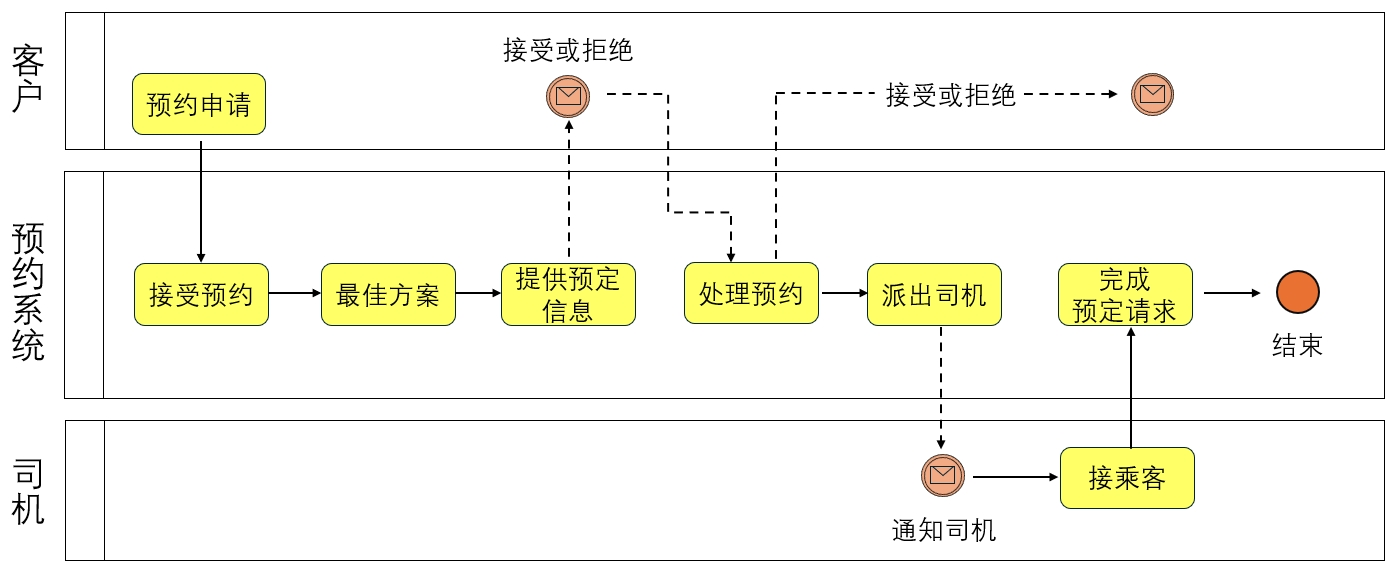
\includegraphics[width=10cm]{6_网约车.jpg}

\begin{enumerate}
\tightlist
\item
  预约申请
\item
  接收预约
\item
  选择最佳方案
\item
  提供预约信息
\item
  处理预约
\item
  分派司机
\item
  接乘客
\item
  完成预约请求
\end{enumerate}

客户：是的，每个行为都要花一定开发工作量。\\
我：其实按SiFP只有4个行为，因开头4个和最后2个都要合并才正确（详见附件），因如果要能独立成行为，必须符合基本过程条件。\\
基本过程不是随便定的，它有规则，比如从网约车案例我们可以看到，``预约申请''本身不能算一个基本过程，虽然预约申请可能要很复杂的开发工作，但是因为它不能独立存在，必须依赖其他的行为才算完整。\\
例如某公司财务系统有打印支票功能（用来付供应商），你觉得打印支票本身是否算基本过程？\\
客户：听完你网约车例子，应该不算。因打印支票只是付款流程的一部分。\\
我：正确，好比银行账户转账，更新账户余额
和展示账户余额这3个用例不能单独，必须合起来才算完整。算实体也应使用同样概念。例如某人事管理系统，除了管理职工信息外，还有员工家属信息，因家属信息必须关连到员工信息，不能独立存在，所以家属信息本身不算是一个实体。你是否觉得你这表里的某些实体应合并？\\
客户：听完你的解释，我们这次计算里确实有些实体应合并。\\
但如果客户需要管理员工家属信息，我们在建数据库时确实要增加额外表格管理相关的字段，会增加不小工作量，所以如果和只需要管理员工信息，同样是算一个实体，同样的功能点数，是否不合理？\\
我：很理解你的疑问，也正是很多工程师功能点的困惑。
你在之前不是说过在估算开发工作量时常常与客户谈不拢，客户常常觉得你们估算的工作量过大大，应不需要这么多。
所以功能点估算的目的是希望从客户的角度，依据功能需求，按已定的规则，让任何人都能算出同样的动能点数（不仅依赖工程师估算）。
所以有些工程师学功能点时，像你一样未能抛开软件开发工作量的想法，不觉得应只按功能点的规则来计算。\\
客户：理解你的意思，但你刚才这个例子确实有额外的工作量，是否导致会低估了项目的工作量？\\
我：预算工作量除了考虑功能点也要看团队的历史生产率数据。
如果以往项目里，很多实体都比较复杂，都包含几个相关的数据表，反映在项目的生产率历史数据里，
作为新项目工作量估算的参考。\\
我：你们的功能点估算表没有明确区分新的迭代怎么处理变更与删除。\\
客户：我们表中有计算每次迭代的总功能点数。\\
我：你们可能有计算每迭代的功能点，但难以看清后面迭代对应之前的变化。优化余维护(Enhancement)功能点是用来估算本迭代的工作量，而应用(Application)功能点就是迭代后产品的功能点数。而且应该用表格形式把变更和删除累加在原本上一轮的功能上面，才可以更好看到迭代与迭代之间功能上的变化。\\
所以不要误以为可以像之前故事点估算，按个人理解写上各种不同复杂程度的故事点例子便可。国际功能点手册里包含很多计算实例，来解释功能点计算，才能确保对同一套功能需求，每人都能估算出同样的功能点数。我刚刚的例子全都可以从国际功能点手册里找到，你们不需要自己研究再`发明'公式。学功能点估算与写程序类似，必须多动手试，例如按我发你们的6个案例，按案例的功能需求，计算SiFP功能点数。\\
（大家也可以看附件里有2个简单案例：

\begin{enumerate}
\tightlist
\item
  首次开发：管理潜在客户（公司和联系人）信息
\item
  优化功能与维护：首次开发后，添加帮助(Help)页功能，和添加报表
\end{enumerate}

）

\hypertarget{ux603bux7ed3}{%
\subsubsection{总结}\label{ux603bux7ed3}}

虽然简化功能点(SiFP)比传统国际功能点（IFPUG）简单易学，但开发人员还是容易用工程师的视角来估算（本应用用户的视角），导致计算错误。所以要多看案例并做练习，才能把握（能参加培训会更好）。

\hypertarget{ux9644ux4ef6}{%
\section{附件}\label{ux9644ux4ef6}}

\hypertarget{ux7b80ux5316ux529fux80fdux70b9sifp-ux7b80ux4ecb}{%
\subsection{简化功能点(SiFP)
简介}\label{ux7b80ux5316ux529fux80fdux70b9sifp-ux7b80ux4ecb}}

 \textbf{它是做什么的？} \\
应用软件开发的客户需求可分成3类：

\begin{enumerate}
\tightlist
\item
  功能性需求
\item
  技术需求
\item
  质量需求
\end{enumerate}

第二类和第三类归为非功能性需求。功能点主要是针对功能性需求，目的是提供对客户有意义的功能点数，来客观地衡量软件规模。

 \textbf{该如何去做？} \\
简化功能点(SiFP)主要分为两类度量：

\begin{enumerate}
\tightlist
\item
  数据功能------实体 (逻辑文件 Logical File)
\item
  交易功能------行为（基本过程 Elementary Process)
\end{enumerate}

%\href{文件:微信截图_20241023102406.jpg}{600px}

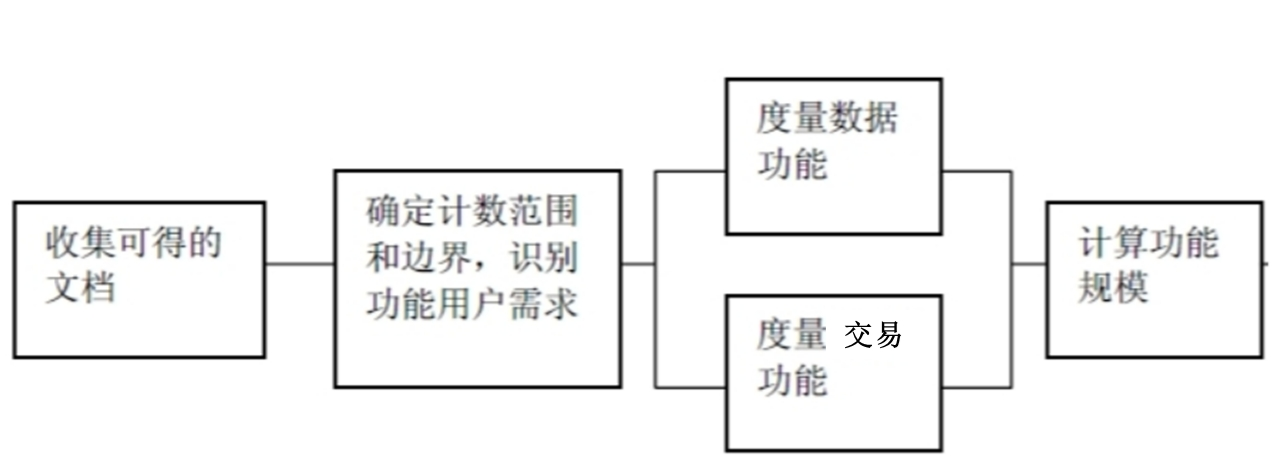
\includegraphics[width=10cm]{微信截图_20241023102406.jpg}

\hypertarget{ux7b80ux5316ux529fux80fdux70b9ux4f30ux7b97ux6b65ux9aa4}{%
\subsubsection{简化功能点估算步骤：}\label{ux7b80ux5316ux529fux80fdux70b9ux4f30ux7b97ux6b65ux9aa4}}

\begin{enumerate}
\tightlist
\item
  确定功能点分析类型
\item
  识别分析范围和应用边界
\item
  计算数据类型功能点
\item
  计算交易类型功能点
\item
  计算功能点
\end{enumerate}

\hypertarget{ux786eux5b9aux529fux80fdux70b9ux5206ux6790ux7c7bux578b}{%
\subsubsection{1
确定功能点分析类型}\label{ux786eux5b9aux529fux80fdux70b9ux5206ux6790ux7c7bux578b}}

3种计算类形：

\begin{enumerate}
\tightlist
\item
  开发(Development )
\item
  优化功能与维护 (Functional Enhancement Maintenance FEM)
\item
  应用 (Application)
\end{enumerate}

开发(Development
)功能点数包括首次应用开发的功能点，加上数据迁移或转换的功能点。

优化功能与维护 (FEM)
计算对现有应用软件的优化与维护，包括增加、删除和变更功能，也加上数据迁移或转换的功能点。

应用
(Application)计算已经安装应用软件，例如优化与维护后的软件，提供给用户的功能点数，

\hypertarget{ux8bc6ux522bux5206ux6790ux8303ux56f4ux548cux5e94ux7528ux8fb9ux754c}{%
\subsubsection{2
识别分析范围和应用边界}\label{ux8bc6ux522bux5206ux6790ux8303ux56f4ux548cux5e94ux7528ux8fb9ux754c}}

IFPUG 包括两类数据功能点 （因SiFP 是基于IFPUG 功能点）：

\begin{itemize}
\tightlist
\item
  内部逻辑文件(ILF)
\item
  外部接口文件(EIF)
\end{itemize}

和3类交易类功能点：

\begin{itemize}
\tightlist
\item
  外部输入 (EI)
\item
  外部输出 (EO)
\item
  外部查询 (EQ)
\end{itemize}

以下例子表示数据类和交易类功能点与应用软件系统（参考案例A）的关系（虚线标示系统边界）：\\
%\href{文件:微信截图_20241024151135.jpg}{600px}\\

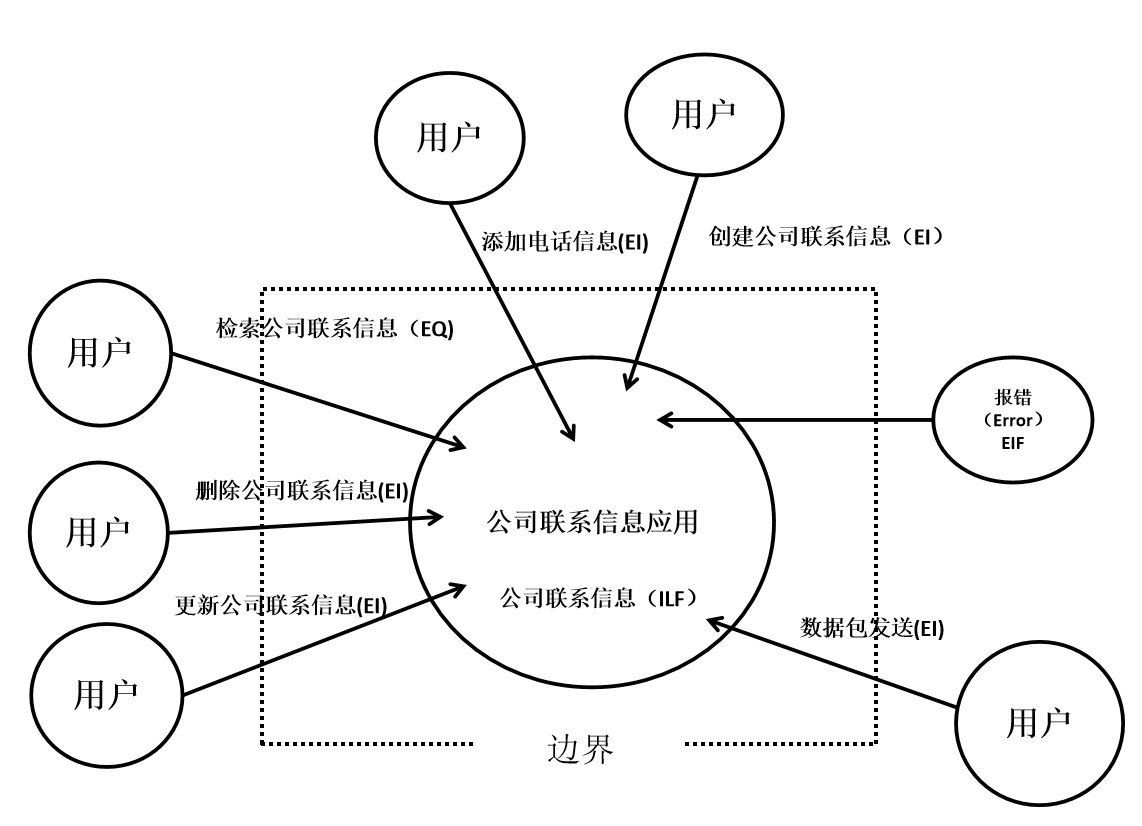
\includegraphics[width=10cm]{微信截图_20241024151135.jpg}

\begin{description}
\tightlist
\item[]
= = = =
\end{description}

%\href{文件:微信截图_20241023102437.jpg}{600px}

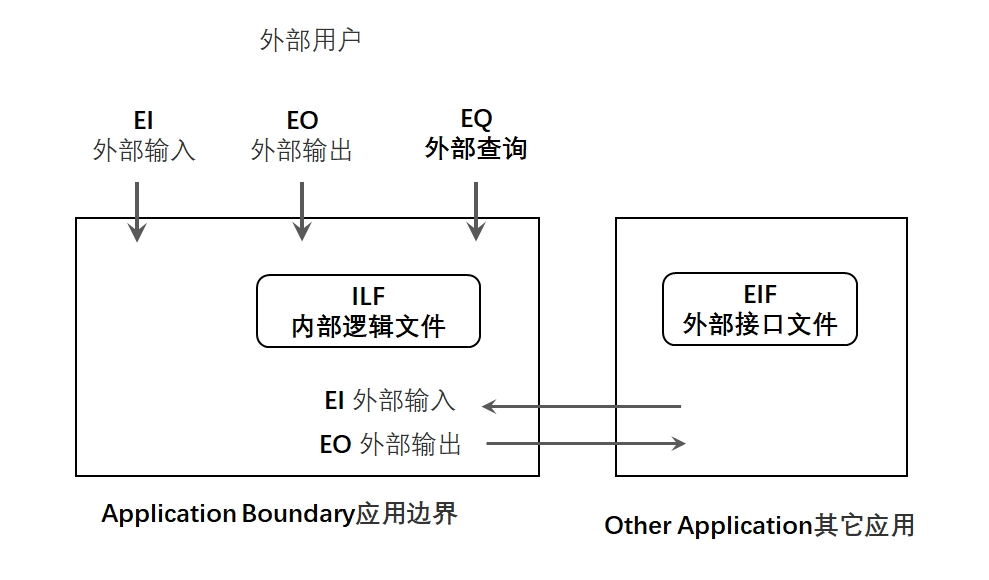
\includegraphics[width=10cm]{微信截图_20241023102437.jpg}

计数范围由计数目的决定。它标识将被划分大小的系统、应用程序或应用程序的子集。它可以包括通过购买软件包来满足的功能；它可以包括所有将被外包的应用程序；它可以被限制为应用程序中执行特定目的的函数，例如报表。应用程序边界是被测量的应用程序与外部应用程序或用户域之间的边界。

IFPUG制定了确定边界的具体规则：

\begin{itemize}
\tightlist
\item
  \textbf{边界是基于用户的观点}
  用户应该能够用用户的语言定义应用程序的范围和业务功能
\item
  \textbf{相关应用程序之间的界限是基于单独的业务功能，而不是基于技术考虑}
  举例，微软办公软件目前包括Word、Excel、PowerPoint 和 Access；每个都是
  Microsoft office 套件中的独立应用程序
\item
  \textbf{被增强的应用程序的应用程序边界保持原样}
  当然，除了添加的功能可能会扩展边界，删除的功能可能会缩小边界。功能优化不会成为它自己的应用边界，而是按计数应用程序的领域定义（如微服务）。如开发项目和优化项目可能包括不止一个应用程序，功能点计数时应参考上图例子先画好边界，然后独立计算每个应用程序的功能点数
\end{itemize}

有关应用程序中制定3边界定义的混淆。\\
虽然功能点计算的一致性非常重要，但如果计算一致但不正确，功能点计算几乎没有什么好处。例如，在确定应用程序边界时。边界不应该在软件程序或软件模块级别建立。功能点似乎只在更高的应用程序级别上才相关。

\begin{itemize}
\tightlist
\item
  但也可能在过高的层次上进行计数，例如，某会计系统可能包含几个独特的和独立的应用程序（例如，应收帐款、总账和应付帐款），它们可能具有内部关系。这些应用程序应该分别计算
\item
  反过来，某工厂生产系统可以由许多从属但独立的应用程序（例如，车间计划，物料库存，工作计划）组成，这些应用程序分别开发，维护和使用，并且可能具有内部关系
\end{itemize}

\hypertarget{ux8ba1ux7b97ux6570ux636eux7c7bux578bux529fux80fdux70b9}{%
\subsubsection{3
计算数据类型功能点}\label{ux8ba1ux7b97ux6570ux636eux7c7bux578bux529fux80fdux70b9}}

\begin{itemize}
\tightlist
\item
  先计算逻辑文件数
\item
  关于计算规则，详见``逻辑文件''
\item
  按对应公式计算功能点数 :( 每个逻辑文件 = 7.0 简化功能点）
\end{itemize}

\hypertarget{ux8ba1ux7b97ux4ea4ux6613ux7c7bux578bux529fux80fdux70b9}{%
\subsubsection{4
计算交易类型功能点}\label{ux8ba1ux7b97ux4ea4ux6613ux7c7bux578bux529fux80fdux70b9}}

\begin{itemize}
\tightlist
\item
  计算基本过程数
\item
  关于计算规则，详见``基本过程''
\item
  按对应公式计算功能点数 :( 每个逻辑文件 = 7.0 简化功能点 ；每个基本过程
  = 4.6 简化功能点）
\end{itemize}

\hypertarget{ux8ba1ux7b97ux529fux80fdux70b9}{%
\subsubsection{5 计算功能点}\label{ux8ba1ux7b97ux529fux80fdux70b9}}

\begin{itemize}
\tightlist
\item
  功能点数 = 数据类型功能点数 + 交易类型功能点数
\end{itemize}

\hypertarget{development-project-function-point-count-ux5f00ux53d1ux9879ux76eeux529fux80fdux70b9ux8ba1ux6570}{%
\subsubsection{Development Project Function Point Count
开发项目功能点计数}\label{development-project-function-point-count-ux5f00ux53d1ux9879ux76eeux529fux80fdux70b9ux8ba1ux6570}}

开发项目功能点计数由两个功能点数组成：

1. 应用程序的功能点数，由EI、EO、EQ、ILF 和 EIF 组成\\
2.
转换功能，通过软件将以前的数据转移到新的ILF中（该组件通常包括旧数据文件的输入作为EI计数或将数据输入到已计数的新ILF中，可能还包括转换报告的EO）\\

DFP = UFP + CFP

\begin{itemize}
\tightlist
\item
  DFP是开发项目功能点计数。
\item
  UFP为功能点计数。
\item
  CFP是数据转换所包含的功能点的数目。（注1）
\end{itemize}

\hypertarget{enhancement-project-function-point-count-ux4f18ux5316ux7ef4ux62a4ux9879ux76eeux529fux80fdux70b9ux8ba1ux6570}{%
\subsubsection{Enhancement Project Function Point Count
优化维护项目功能点计数}\label{enhancement-project-function-point-count-ux4f18ux5316ux7ef4ux62a4ux9879ux76eeux529fux80fdux70b9ux8ba1ux6570}}

功能点计数也由两个功能数组成，但它们有些不同：\\
1. 应用程序未调整的功能点计数，由EL、EO、EQ、ILF和ELF组成，它们是：\\
*由增强项目增加(以前不存在的功能，例如：一个新的EQ，三个新的EL，一个新的ILE，一个新的EQ和一个新的EO)

\begin{itemize}
\tightlist
\item
  由增强项目更改（以前存在的功能，但现在有不同的字段，FTR或需要不同的处理）
\item
  由增强项目删除(已从应用程序中删除的功能，例如：已删除的报告)
\end{itemize}

2.
转换功能，通过软件将以前的数据转换为新的ILF（该组件通常包括旧数据文件的输入{[}作为EL计数或将数据输入到已计数的ILF中{]}，可能还包括转换报告的EO）\\
增强项目功能点计算公式如下：

EFP =(ADD + CHGA + CFP) + DEL

\begin{itemize}
\tightlist
\item
  EFP是增强项目功能点计数
\item
  ADD是增强项目增加的功能的未调整功能点数
\item
  CHGA是经增强项目修改的功能的未调整的功能点计数
\item
  CFP是数据转换所包含的功能点的数目（注1）
\item
  DEL 是那些在增强项目中被删除的功能的未调整功能点计数
\end{itemize}

\begin{description}
\tightlist
\item[]
（注1：这简介不包含数据转换的计算与实例。）
\end{description}

\hypertarget{application-function-point-count-ux5e94ux7528ux529fux80fdux70b9ux8ba1ux6570}{%
\subsubsection{Application Function Point Count
应用功能点计数}\label{application-function-point-count-ux5e94ux7528ux529fux80fdux70b9ux8ba1ux6570}}

应用程序功能点计数由一个功能组件组成（转换工作功能不包括在应用程序计数中，因为它是开发工作的一部分，而不是应用程序一旦建立）：

1. 应用程序的功能点计数，包括Els, EOs EQs, ILFs, EIFs

有两种不同的时间段估算应用程序的功能点数：

\begin{enumerate}
\tightlist
\item
  当应用程序最初交付
\item
  当增强项目改变了应用程序的功能值时（当安装增强项目时，必须更新以前的应用程序功能点计数，以识别对应用程序的修改）。增强项目可以修改应用程序
\end{enumerate}

下面是两种不同的计算公式：

\hypertarget{initial-application-function-point-calculation-ux521dux59cbux5e94ux7528ux529fux80fdux70b9ux8ba1ux7b97}{%
\paragraph{Initial Application Function Point Calculation
初始应用功能点计算}\label{initial-application-function-point-calculation-ux521dux59cbux5e94ux7528ux529fux80fdux70b9ux8ba1ux7b97}}

AFP = ADD

\begin{itemize}
\tightlist
\item
  AFP是初始应用程序功能点计数。
\item
  ADD是开发项目所安装功能的未调整功能点数。
\end{itemize}

\hypertarget{application-function-point-calculation-after-an-enhancement-ux4f18ux5316ux4e0eux7ef4ux62a4ux540eux7684ux5e94ux7528ux529fux80fdux70b9ux8ba1ux7b97}{%
\paragraph{Application Function Point Calculation after an Enhancement
优化与维护后的应用功能点计算}\label{application-function-point-calculation-after-an-enhancement-ux4f18ux5316ux4e0eux7ef4ux62a4ux540eux7684ux5e94ux7528ux529fux80fdux70b9ux8ba1ux7b97}}

\begin{itemize}
\tightlist
\item
  增加（新）功能，增加应用程序的功能点大小
\item
  变更，通过增加或减少本来开发功能点，但不影响应用程序的功能点数，只影响了优化维护功能点数
\item
  删除功能，会减少应用程序的功能点，但反而会增加优化维护(Enhancement)功能点。
\end{itemize}

AFP =(UFPB + ADD + CHGA)-(CHGB + DEL)

\begin{itemize}
\tightlist
\item
  AFP是应用程序调整后的功能点计数
\item
  UFPB是增强项目前应用程序的功能点数
\item
  ADD是增强项目增加的功能的未调整功能点数
\item
  CHGA是经增强项目更改的功能的未调整功能点数（此部分反映更改后的功能点值）
\item
  CHGB是改进前未调整的功能点数（此分量反映改进前的功能点值）
\item
  DEL是那些被增强项目删除的功能的未调整功能点计数
\end{itemize}

\hypertarget{ux903bux8f91ux6587ux4ef6-logical-file}{%
\subsection{逻辑文件 (Logical
File)}\label{ux903bux8f91ux6587ux4ef6-logical-file}}

\textbf{下面在计算实例里简称``实体''以方便理解}

\begin{itemize}
\tightlist
\item
  逻辑文件满足内部和外部数据存储要求的功能。它是用户可识别的逻辑相关数据组或控制信息组，
\item
  2类逻辑文件：

  \begin{itemize}
  \tightlist
  \item
    内部逻辑文件(ILF)：在度量应用程序的边界内维护和/或引用。是在被度量应用边界内部维护的
  \item
    外部接口文件(EIF)：被度量应用程序所引用，但在另一应用边界内维护
  \end{itemize}
\end{itemize}

术语定义：

\begin{itemize}
\tightlist
\item
  \textbf{用户可识别（User
  Identifiable）}：对过程和/或数据组的需求，得到用户和软件开发人员双方的认同和理解，并达成一致。例如，财务应用程序可能需要一个支票账户记录\\
\item
  \textbf{逻辑相关（Logically
  related）}：要求每一组与相关描述逻辑上一致。逻辑文件不应为了维持其存在而依赖或归因于另一个逻辑文件，这些相关逻辑文件应合并（特别是因业绩或执行原因而建立的组）。例如，地址表可能属于更高级别，如客户文件、账单文件、库存位置文件或员工文件\\
\item
  \textbf{数据（Data）}:应用程序中维护的描述和/或数据组。例如，每张支票的支票号码、金额、日期、收款人、备忘录记录和账户号码都可能在支票账户记录中维护\\
\item
  \textbf{控制信息（Control
  information）}:应用程序里影响基本过程的数据。它定义处理那些数据(what)、何时处理数据(when)或如何处理数据(how)。对于ILF，这些数据、规则或参数在应用程序中存储和维护。举例，在恒温器上设置温I度以控制加热或空调的时序\\
\item
  \textbf{维护（Maintained）}:通过应用程序的基本过程修改数据。数据或控制数据可以通过诸如添加、更改、删除等。逻辑文件可以被多个应用程序维护，但在每个应用程序只能计算为一个ILF\\
\item
  \textbf{基本过程（Elementary
  process）}:具有意义的最小活动单位。它可以更新多个逻辑文件\\
\end{itemize}

\framebox{%
\begin{minipage}[t]{0.97\columnwidth}\raggedright
注意:\\
逻辑文件包括两类不同的用户需求数据：

\begin{enumerate}
\tightlist
\item
  功能性数据
\item
  非功能性数据\\
\end{enumerate}

功能性数据是用来满足用户功能需求的数据。例如销售、银行账号、供应商、人员等信息。\\
非功能性数据主要是为了满足易用性（如支撑下拉菜单所需的数据，可输入数据的上下范围等），或性能（如用于查询数据的索引），或可维护性（配置参数）。\\
只有第一类功能性数据才算是逻辑文件。\\
功能点估算只包括功能性需求，国际功能点(IFPUG)有SNAP计数手册，专门针对非功能需求。\strut
\end{minipage}}

\hypertarget{ux57faux672cux8fc7ux7a0b-elementary-process-ep}{%
\subsection{基本过程 (Elementary Process
EP)}\label{ux57faux672cux8fc7ux7a0b-elementary-process-ep}}

基本过程是对用户有意义的最小活动单元。例如:添加员工的用户需求包括建立工资和家属信息。只有添加所有员工信息,才能创建员工信息记录。单独添加一些信息使添加员工业务处于不持续状态,只有员工工资和家属信息都添加后,这个活动单元才能完成且业务处于稳定状态。

\hypertarget{ux8bc6ux522bux57faux672cux8fc7ux7a0b}{%
\subsubsection{识别基本过程}\label{ux8bc6ux522bux57faux672cux8fc7ux7a0b}}

为了识别基本过程，需要执行以下活动，把功能用户需求分解为最小活动单元,使其满足下面条件：

\begin{itemize}
\tightlist
\item
  对用户有意义\\
  例如功能用户需求要求在应用中添加新员工的能力
\item
  构成一个完整的事务\\
  例如:用户定义的员工信息包括工资和家属信息。如果家属人数大于零,添加员工信息时必须包括家属信息。本例中,添加员工信息(不包括添加地址、工资和家属信息)不满足本规则
\item
  自包含\\
  例如:除非输入所有的必需信息并且完成所有处理步骤,如验证、计算、更新ILFs,添加过程才是自包含的
\item
  让应用程序的业务保持持续状态\\
  例如添加员工的用户需求包括建立工资和家属信息。只有添加所有员工信息,才能创建员工信息记录。单独添加一些信息使添加员工业务处于不持续状态,只有员工工资和家属信息都添加后,这个活动单元才能完成且业务处于持续状态\\
\end{itemize}

识别活动单元为基本过程需要满足以上所有规则。\\

\hypertarget{ux8bc6ux522bux57faux672cux8fc7ux7a0bux4e3bux8981ux76eeux7684}{%
\subsubsection{识别基本过程主要目的}\label{ux8bc6ux522bux57faux672cux8fc7ux7a0bux4e3bux8981ux76eeux7684}}

基本过程的主要目的可识别为下列情形的一种:

\begin{itemize}
\tightlist
\item
  改变应用行为
\item
  维护一个或多个ILFs
\item
  呈现信息给用户
\end{itemize}

\hypertarget{ux5b9eux4f8bux8bc6ux522bux57faux672cux8fc7ux7a0b-ep}{%
\subsection{实例：识别基本过程
(EP)}\label{ux5b9eux4f8bux8bc6ux522bux57faux672cux8fc7ux7a0b-ep}}

下面是预约网约车过程：

\resizebox{\linewidth}{!}{

\renewcommand{\arraystretch}{1.5}

\begin{tabular}{|c|c|}
\hline
活动名称&描述\\
\hline
预约申请&客户发出预约请求到预约系统，预约信息包括：日期、时间、上车的位置和目的地位置。\\
\hline
接收预约&预约系统收集客户预约请求，并把预约数据记录在数据库。\\
\hline
检查是否有可用的车/司机&预约系统从预约数据库中查看是否有合适的车/司机，如果能找到合适的时间、日期，能配合预约请求的话，看看司机是否有空档。如能找到，在系统更新内部状态为是，否则为否。 \\
\hline
寻找其他可选&如果状态是没有，预约系统继续在数据库搜索有没有接近的预期时间，否则写没有合适请求的出发地点和目的地。 \\
\hline
提供预约信息&预约系统自动发出通知到客户，是否有合适空档或者提供接近的日期时间。 \\
\hline
处理预约&客户回复预约系统接受或拒绝，预约系统把反馈记录在预约数据库。如果反馈是接受，预约系统会继续统计客户详细预约信息。如果客户拒绝，预约系统就会回复收到，并终止过程。 \\
\hline
分派司机&如果客户接受，预约系统会指派司机到已确认的日期、时间、上车地点和目的地。预约系统把这个记录在数据库中，并发信息通知相关司机。 \\
\hline
接乘客&司机按约好的日期时间、上车的地点接乘客，然后发信息到预约系统，通知乘客已经上车。\\
\hline
完成预约请求&预约系统在数据库中记录已经完成整个过程。\\
\hline
\end{tabular}

}

\textbf{分析能否满足所有 EP 识别规则，判断能否独立成为基本过程
(EP),部分例子}

\hypertarget{ux9884ux7ea6ux7533ux8bf7}{%
\subsubsection{预约申请}\label{ux9884ux7ea6ux7533ux8bf7}}

\begin{enumerate}
\tightlist
\item
  是否对用户有意义，是客户功能需求的一部分。\textbf{是}
\item
  是否构成一个完整的事务？\textbf{否}：预约申请本身不是一个完整的交易，因为过程必须也包括预约请求信息，收到其他可选的档期这些步骤，都不可以分离
\item
  是否自包含，可以独立存在？\textbf{否}：例如接受预约申请，查看是否有档期，查看有没有其他接近的档期等，都是一些必需的相关步骤去完成这个基本过程
\item
  是否让应用程序达到稳定状态？\textbf{否}：整个业务需求只能在收到预约信息，发送、接受、处理、反馈给客户才算是完成稳定状态
\end{enumerate}

\hypertarget{ux5206ux6d3eux53f8ux673a}{%
\subsubsection{分派司机}\label{ux5206ux6d3eux53f8ux673a}}

\begin{enumerate}
\tightlist
\item
  是否对用户有意义，是客户功能需求的一部分。\textbf{是}
\item
  是否构成一个完整的事务？\textbf{是}：分配到司机是一个完整的交易，包括收到司机的确认，把信息记录在系统中并通知司机
\item
  是否自包含，可以独立存在？\textbf{是}：分配到司机本身可以独立存在
\item
  是否让应用程序达到稳定状态？\textbf{是}：因为当司机被分配后，是完全满足业务的需要
\end{enumerate}

\hypertarget{ux63a5ux4e58ux5ba2}{%
\subsubsection{接乘客}\label{ux63a5ux4e58ux5ba2}}

\begin{enumerate}
\tightlist
\item
  是否是客户功能需求？\textbf{是}
\item
  交易是否完整？\textbf{否}：接乘客本身不算一个完整的交易，因为预约系统必须也记录这个信息
\item
  是否自包含，可以独立存在？\textbf{否}：确认预约申请是下面一个必须执行的过程，来完成这个基本过程
\item
  是否让应用程序达到稳定状态？\textbf{否}：整个业务需求只能在预约系统确认沟通，已经接到乘客，然后系统也把记录更新到预约系统才算完成
\end{enumerate}

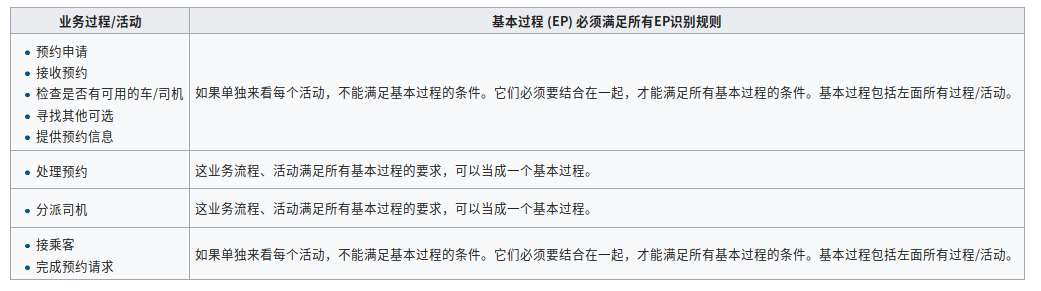
\includegraphics[width=10cm]{Screenshotfrom2023-11-1302-05-21.png}

\hypertarget{ux6848ux4f8baux5f00ux53d1developmentux9879ux76ee}{%
\subsection{案例A:开发(Development)项目}\label{ux6848ux4f8baux5f00ux53d1developmentux9879ux76ee}}

公司计划构建应用程序来维护对其功能点课程感兴趣的公司信息。

要维护的公司联系信息，按逻辑分组，包括以下数据：

\begin{itemize}
\tightlist
\item
  公司
\item
  联系人姓名
\item
  职位
\item
  初次联系日期
\item
  街道地址
\item
  城市
\item
  状态
\item
  邮政编码
\item
  电话号码
\item
  传真号码
\end{itemize}

该数据最初将在收到查询表示对课程感兴趣时创建。员工将能够通过屏幕，使用以下命令创建、更新和删除信息。创建和更新将维护以上所有的10个字段。删除只需要输入公司和联系人的姓名。

下面是公司联系数据中包含的其他字段，但要用另外单独更新：

\begin{itemize}
\tightlist
\item
  发送材料日期
\item
  电话联系日期
\item
  笔记、备注
\end{itemize}

这些字段将由两个独立的基本流程维护：\\
(1)发送信息包时，发送信息包的个人将使用一个单独的屏幕，使用功能键输入公司、联系人姓名和发送数据包的日期。\\
(2)邮件寄出后两周内，回电确认收到并答复问题。合同完成后，来电者将使用屏幕，使用功能键输入联系人的公司名称、电话联系日期和备注。电话联系人的日期将用作辅助键（第二种记录类型），以保存多次出现的信息并更新公司联系人数据。

由菜单驱动的用户界面导航，提供以下六个功能：

\begin{itemize}
\tightlist
\item
  创建公司联系人
\item
  检索公司联系
\item
  更新公司联系
\item
  删除公司联系
\item
  已发送的材料包
\item
  已完成的电话联络
\end{itemize}

除了检索公司联系之外，其他所有功能都已经描述。输入公司、联系人姓名和功能键后，检索功能便显示公司联系数据中维护的所有字段。

任何功能都可以从外部维护的错误（Error）文件返回错误信息，该文件有四个字段，其中一个字段包含具体错误信息。

\hypertarget{ux7b54ux6848ux4e0eux89e3ux8bfb}{%
\subsection{答案与解读}\label{ux7b54ux6848ux4e0eux89e3ux8bfb}}

共个实体：

\begin{enumerate}
\tightlist
\item
  公司联系信息
\item
  报错文件\\
\end{enumerate}

你可能会问：那些电话信息是否也应该是一个实体？（因需要花工夫开发）\\
这不应该是一个实体。因为电话信息必须依赖公司联系信息挂在一起，不可以独立存在，就好比我们要电话信息，假如也要维公司联系信息，这个电话信息就不能算另外一个实体，因为没有公司联系信息，电话信息是不能单独存在的。区分原则不是根据是否要产生开发的工作量，而是从用户角度看，这个实体能否独立存在和维护。否则功能点的估算就只是根据个人对开发工作量的估计，而不是从用户角度看功能的客观判断。\\
创建、检索、更新、删除等4个功能和管理发送资料包和电话联系2功能，共
6行为，加2实体。为方便理解，建议先画下图，把行为与实体关联：

%\url{文件:答案与解读1.1.jpg}

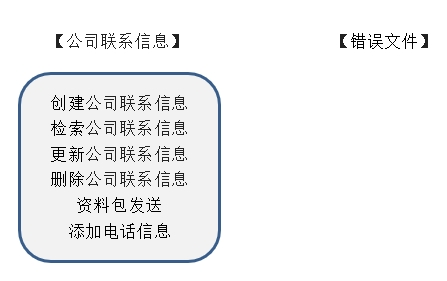
\includegraphics[width=3cm]{答案与解读11.jpg}

所以按简化功能点每个实体×7，每行为×4.6得出
41.6(=2×7+6×4.6)简化功能点，详见下面列表：

%\href{文件:微信截图_20241021091913.jpg}{500px}

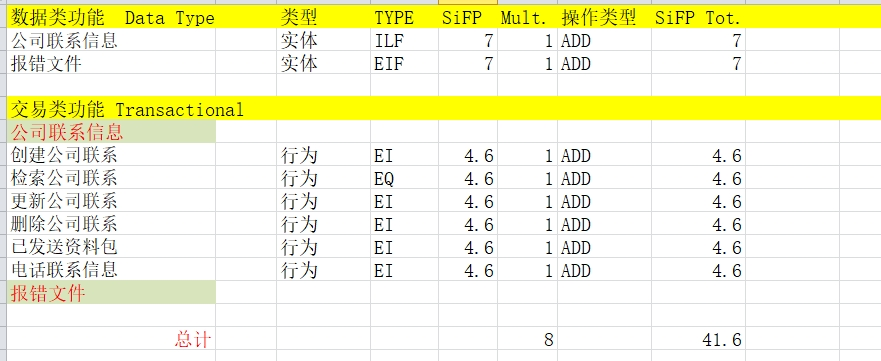
\includegraphics[width=3cm]{微信截图_20241021091913.jpg}

\hypertarget{ux6848ux4f8bbux4f18ux5316ux7ef4ux62a4femux9879ux76ee}{%
\subsection{案例B:优化维护（FEM）项目}\label{ux6848ux4f8bbux4f18ux5316ux7ef4ux62a4femux9879ux76ee}}

应用程序交付后，Caren Garmus
希望利用已经由外部应用程序维护的帮助子系统来提供两类帮助页面：

\begin{enumerate}
\tightlist
\item
  字段级
\item
  屏幕级
\end{enumerate}

每个屏幕上都可用这两个级别的帮助功能，并且将从单独维护的外部帮助文件访问帮助文本。

在所有情况下，Help都少于5个字段。

Mary Herron说她想要一份每周的逾期联系报告（详见下表），识别出：

\begin{itemize}
\tightlist
\item
  那些联系没有收到资料包
\item
  那些在邮寄后两周内没有接到电话联系
\end{itemize}

该报告将每周从公司联系数据文件中检索数据，不需要更改公司联系数据文件。

\framebox{%
\begin{minipage}[t]{0.97\columnwidth}\raggedright
\toprule
日期： xxxx.xx.xx 页码：xx\tabularnewline
\midrule
\endhead
从 xxxx.xx.xx :\tabularnewline
公司\tabularnewline
联系人\tabularnewline
首次联系日期\tabularnewline
数据包发送 xxxx.xx.xx\tabularnewline
计划电话联系日期 xxxx.xx.xx\tabularnewline
过期总数\tabularnewline
\bottomrule
\strut
\end{minipage}}

\hypertarget{ux7b54ux6848ux4e0eux89e3ux8bfb-1}{%
\subsection{答案与解读}\label{ux7b54ux6848ux4e0eux89e3ux8bfb-1}}

另外加了一个要管理的实体：

\begin{enumerate}
\tightlist
\item
  帮助文件\\
\end{enumerate}

也可参考IFPUG关于ILF/EIF (实体)的识别要求，必须符合以下条件：

\begin{enumerate}
\tightlist
\item
  数据的集合必须是逻辑相关的并且是用户可以识别
\item
  这些数据或者控制信息必须是在本应用的边界内被维护\\
\end{enumerate}

总结：

\begin{itemize}
\tightlist
\item
  实体方面增加了1个实体，
\item
  行为增加4个行为\\
\end{itemize}

所以动态功能点是增加的功能点25.4 (=1×7 +4×4.6)

%\href{文件:微信截图_20241024094600.jpg}{700px}

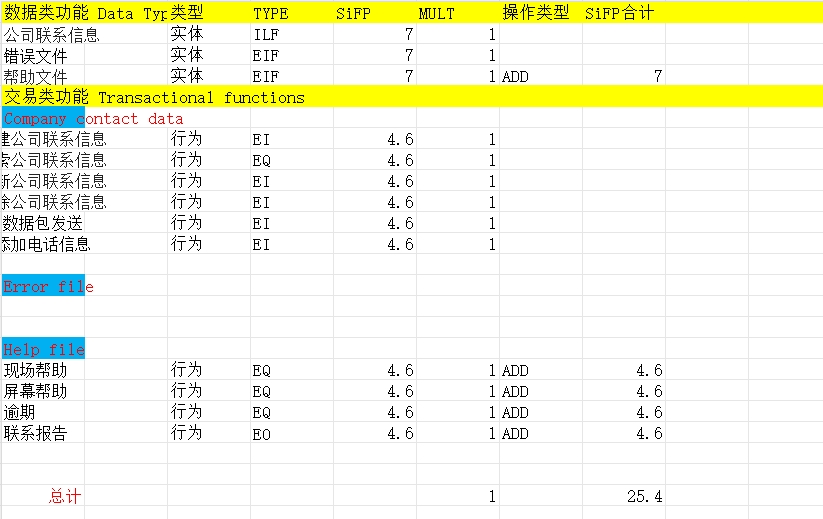
\includegraphics[width=10cm]{微信截图_20241024094600.jpg}

\hypertarget{ux4e0eux56fdux9645ux529fux80fdux70b9ifpugux7684ux504fux5dee}{%
\subsection{与国际功能点(IFPUG)的偏差}\label{ux4e0eux56fdux9645ux529fux80fdux70b9ifpugux7684ux504fux5dee}}

以案例A为例子：

\begin{itemize}
\tightlist
\item
  使用IFPUG数EI、EO、EQ、ILF、EIF
  每类都有规则判断复杂度，高中低，对应得出功能点数。例如ILF公司联系信息可分成2组，公司信息和联系信息如打电话、资料包等；总共包括13类字段，数据组
  (Record Elements Type RET) =2, 字段(Data Element Types DET)
  =13，ILF复杂度为低。同样思路，创建、查询、更新也都是2组共不超过15
  DET字段，按定义都是属于中等，但删除只需要共4字段，所以复杂度低，加起来得出调整前功能点数FP=35
  (详见下表）
\item
  使用SiFP估算实体和行为数，计算得出FP=41.6
\end{itemize}

%\href{文件:115页替换图片.jpg}{600px\textbar{}无}

%\href{文件:微信截图_20241023163812.jpg}{700px}

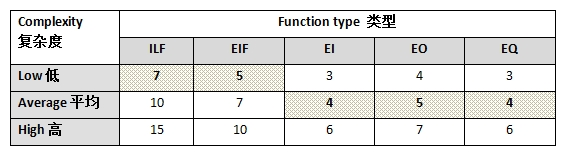
\includegraphics[width=10cm]{115页替换图片.jpg}

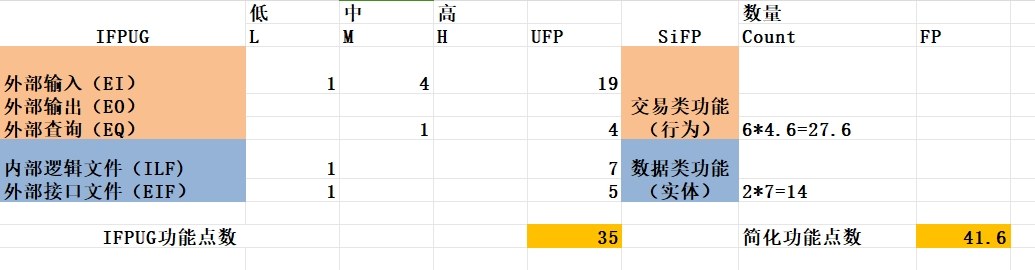
\includegraphics[width=10cm]{微信截图_20241023163812.jpg}

\begin{itemize}
\tightlist
\item
  SiFP得出的实体数量，与行为数量都一样（实体(=ILF+EIF)=2；行为(=EI+EO+EQ)=6）
\item
  因为简化功能点只是不区分实体与行为的复杂度(高中低)，取平均值。因这案例A复杂度偏低，所以用IFPUG考虑复杂度时功能点数比SiFP低，但如果综合公司多个项目，复杂度有高有低，平均的差异便会降低
\end{itemize}

\hypertarget{ux53c2ux8003references}{%
\section{参考References}\label{ux53c2ux8003references}}

\begin{enumerate}
\tightlist
\item
  Brigido, Sergio. "FPA Rules interpretations for Elementary Processes "
  , IFPUG Whit paper. (2022)\\
\item
  SiFPA Assoc. "Simple Function Point Functional Size Measurement
  Method, Measurement Examples " , SiFP-0.1.00-EX-EN-01.01 (2014)\\
\item
  Garmus, David. 'Function Point Analysis' , Addison-Wesley (2001)
\end{enumerate}



\end{document}
